\section{Complementary vertices, prismatoids, and packing polytopes}\label{sec:geometry}

The distant vertices of Theorem~\ref{thm:main} can be made
\emph{complementary}, meaning that each facet contains exactly one of them.
A simple $d$-polytope with such a pair has exactly $2d$ facets.
The wedge of Klee and Walkup~\cite{kw} lets us assign an uncovered facet
to the two vertices without shortening the distance between them.

\begin{corollary}[Complementary vertices]\label{cor:spindle}
For every prescribed positive integer function $s(d)=d^{o(1)}$ and all
sufficiently large $d$, a rational simple $d$-polytope with $2d$ facets
has complementary vertices at $s(d)$-move distance $d^{\omega(1)}$.
\end{corollary}

\begin{proof}
Start with the polytope of Theorem~\ref{thm:main} having $d$ facets and
move allowance $s(d)$. Let $v,w$ be two distant vertices and let $F$ be
the smallest face containing both. Every face of $F$ is a face of the
original polytope, so restricting to $F$ preserves the distance lower
bound. In its affine hull $F$ is rational and simple. Write $p=\dim F$
and let $m\le d$ be its facet count. Each of $v,w$ lies on $p$ facets
of $F$, and no facet of $F$ contains both. Thus $m-2p$ facets of $F$
contain neither vertex.

Choose such a facet with rational affine slack $a(x)$. The wedge is
\[
               W=\{(x,t):x\in F,\ 0\le t\le a(x)\}.
\]
Its bottom and top sheets replace the chosen facet, and every other
facet of $F$ lifts to a facet of $W$. A vertex above a vertex of $F$
with $a(x)>0$ belongs to one sheet and $p$ lifted facets. When
$a(x)=0$, the single vertex above it belongs to both sheets and
$p-1$ lifted facets. This list exhausts the vertices, since each sheet is an
affine copy of $F$, and an interior point of a fiber can move along
that fiber. Hence $W$ is a rational simple $(p+1)$-polytope.

Consider any face of $W$ maximizing $b\cdot x+ct$. Maximizing first
over the fiber gives $b\cdot x+\max(c,0)a(x)$, an affine function of
$x$. The projection of the face is therefore a face of $F$, of
dimension at most that of the original face. Every allowed move of
wedge vertices projects to an allowed move or a stationary step.

Lift $v$ to the bottom sheet and $w$ to the top. Both vertices had
positive slack in the chosen facet, so each new sheet contains just one
of the two lifted tips. The incidence of the other facets with $v,w$ is
preserved. Repeating the operation $m-2p$ times produces complementary
vertices in dimension $m-p\le d$. Take the product with a cube of
dimension $d-(m-p)$ and choose opposite cube vertices over the tips.
Every product face projects to a face of the first factor. This gives
complementary vertices in dimension $d$ with the required distance.
\end{proof}

\subsection{Two simplex bases and their middle section}

Translate the midpoint of the complementary vertices to the origin.
It is interior, since a supporting facet through it would contain both
vertices. In the polar $T$, the two vertices correspond to facets
$T_0,T_1$ with opposite normals. Each vertex of $T$ lies on exactly one
of these facets. Thus $T$ is a rational simplicial \emph{prismatoid},
the convex hull of two simplex bases in parallel hyperplanes. For
$1\le s<d$, let an $s$-step between facets join two that share a nonempty
face of codimension at most $s$ within each facet. A primal face of
dimension $j$ containing two vertices corresponds to a face of
codimension $j$ within their dual facets. Hence the $s$-step distance
$D_s$ between $T_0,T_1$ equals the primal $s$-move distance between
the tips. For $s=1$, this is the \emph{width} of the prismatoid, measured
by adjacency across ridges~\cite{santos}.

\begin{corollary}[Minkowski sum of two simplices]\label{cor:minkowski}
For every positive integer function $s(d)=d^{o(1)}$ and all sufficiently
large $d$, there are rational $(d-1)$-simplices $U,V$ in
$\mathbb R^{d-1}$ for which two facets of $U+V$ require $d^{\omega(1)}$
$s(d)$-steps. The sum has at most $d^2$ vertices, and each proper
nonempty face is affinely isomorphic to a product of two simplices,
allowing point factors.
\end{corollary}

\begin{proof}
Choose rational affine coordinates in which the bases are $(U,0)$ and
$(V,1)$. In a convex combination at height $1/2$, the coefficients of
the vertices on each base sum to $1/2$. The middle hyperplane $H$
therefore cuts $T$ in a copy of $(U+V)/2$, the section construction of
Santos~\cite[Proposition~5.1]{santos}. Figure~\ref{fig:prismatoid}
illustrates the correspondence between the section facets and the
lateral facets of $T$.

\begin{figure}[htbp]
\centering
\definecolor{sectionink}{RGB}{40,82,94}
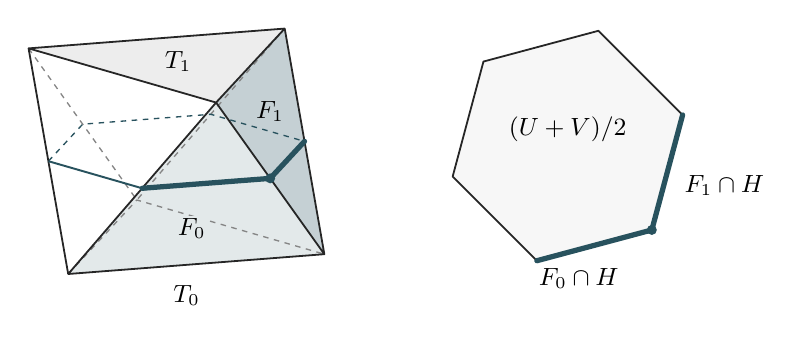
\begin{tikzpicture}[x=1.08cm,y=1.08cm,font=\small,line join=round,
    edge/.style={draw=black!85,line width=.65pt},
    hidden/.style={draw=black!48,line width=.48pt,dash pattern=on 2pt off 2pt},
    cut/.style={draw=sectionink,line width=.7pt},
    walk/.style={draw=sectionink,line width=1.9pt,line cap=round}]
  % View of a triangular antiprism with a horizontal middle section.
  \coordinate (u0) at (-1.273,-.368);
  \coordinate (u1) at (1.739,-.135);
  \coordinate (u2) at (-.466,.502);
  \coordinate (v0) at (.466,1.648);
  \coordinate (v1) at (1.273,2.518);
  \coordinate (v2) at (-1.739,2.285);
  \path (u0) -- coordinate[midway] (p1) (v0);
  \path (u1) -- coordinate[midway] (p2) (v0);
  \path (u1) -- coordinate[midway] (p3) (v1);
  \path (u2) -- coordinate[midway] (p4) (v1);
  \path (u2) -- coordinate[midway] (p5) (v2);
  \path (u0) -- coordinate[midway] (p6) (v2);
  \fill[black!7] (v0) -- (v1) -- (v2) -- cycle;
  \fill[sectionink!13] (u0) -- (u1) -- (v0) -- cycle;
  \fill[sectionink!27] (u1) -- (v1) -- (v0) -- cycle;
  \draw[hidden] (u0) -- (u2) -- (u1) (v2) -- (u2) -- (v1);
  \draw[hidden,sectionink] (p6) -- (p5) -- (p4) -- (p3);
  \draw[edge] (u0) -- (u1) -- (v1) -- (v2) -- cycle
    (u0) -- (v0) -- (u1) (v2) -- (v0) -- (v1);
  \draw[cut] (p6) -- (p1);
  \draw[walk] (p1) -- (p2) -- (p3);
  \fill[sectionink] (p2) circle (1.8pt);
  \node at (.02,2.13) {$T_1$};
  \node[fill=sectionink!13,inner sep=1pt] at (.18,.17) {$F_0$};
  \node[fill=sectionink!27,inner sep=1pt] at (1.10,1.54) {$F_1$};
  \node[below] at (.12,-.39) {$T_0$};
  % View of the same section from above, aligned left-to-right.
  \begin{scope}[shift={(4.60,1.14)}]
    \coordinate (q1) at (-.362,-1.352);
    \coordinate (q2) at (.990,-.990);
    \coordinate (q3) at (1.352,.362);
    \coordinate (q4) at (.362,1.352);
    \coordinate (q5) at (-.990,.990);
    \coordinate (q6) at (-1.352,-.362);
    \filldraw[fill=black!3,edge] (q1) -- (q2) -- (q3) -- (q4) --
      (q5) -- (q6) -- cycle;
    \draw[walk] (q1) -- (q2) -- (q3);
    \fill[sectionink] (q2) circle (1.8pt);
    \node at (0,.19) {$(U+V)/2$};
    \node[below] at (.13,-1.33) {$F_0\cap H$};
    \node[anchor=west] at (1.26,-.47) {$F_1\cap H$};
  \end{scope}
\end{tikzpicture}
\caption{The middle plane $H$ cuts a triangular antiprism in a hexagon.
The lateral facets $F_0,F_1$ meet along an edge with one endpoint
on each base. Its midpoint is the common vertex of the two highlighted
section edges. The three-step walk $T_0,F_0,F_1,T_1$ thus gives the
one-step walk $F_0\cap H,F_1\cap H$ in the section.}
\label{fig:prismatoid}
\end{figure}


At a relative interior point of a nonempty section face $G$, the tight
facet inequalities determine a unique face $\widetilde G$ of $T$.
Intersecting those equalities with $H$ gives $G$ again. Conversely, a
face with vertices on both bases meets $H$ in its relative interior
and loses exactly one dimension on slicing. This correspondence
preserves inclusions and codimensions within lateral facets.

Let $\mathcal A_i(s)$ be the facets of the section whose lifts have at
least $d-s$ vertices on $T_i$. A lateral facet is a simplex, so this
vertex condition says precisely that the facet is one $s$-step from
$T_i$. We claim that
\[
  \operatorname{dist}_s\bigl(\mathcal A_0(s),\mathcal A_1(s)\bigr)=D_s-2,
\]
where the left side is the minimum facet-to-facet distance in the
section. Any section walk lifts to a lateral walk with the same
codimension at each step. Adding the two base facets gives the lower
bound $D_s-2$ on its length. For the reverse inequality, take a
shortest walk from $T_0$ to $T_1$. Two successive lateral facets on
this walk share at least $d-s$ vertices. If their entire intersection
lay in $T_0$, the second facet could be reached in one step directly
from $T_0$. If it lay in $T_1$, the first could step directly to
$T_1$. Either shortcut would shorten the walk. Hence each such
intersection cuts $H$ in the same codimension within the section
facets. The interior of the walk descends to a section walk of length
$D_s-2$. Taking $s=s(d)$ gives the asserted distance.

The Minkowski sum is the convex hull of the $d^2$ pairwise vertex
sums. The lift of any proper nonempty section face is a simplex.
Its barycentric coordinates on $H$ are two nonnegative vectors, one
for each base, each with sum $1/2$. Thus the face is affinely a
product of the two simplices of these barycentric vectors.
\end{proof}

\paragraph{A regular triangulation of large depth.}
Project through $T_0$ from a rational viewpoint just beyond that facet
and strictly beneath all the others. In this Schlegel diagram~\cite{ziegler},
the remaining facets triangulate the $(d-1)$-simplex $T_0$. The
$d$ images of the vertices of $T_1$ are interior and span one maximal
simplex. To see that the triangulation is regular, place the viewpoint
at $(0,-1)$ and the base at height $z=0$, with $T$ in $z\ge0$.
The rational projective map
\[
       (x,z)\longmapsto \bigl(x/(1+z),-z/(1+z)\bigr)
\]
takes the sight lines to vertical lines. Write $(X,Z)$ for the new
coordinates. A non-base inequality $a\cdot x+bz\le c$ becomes
$a\cdot X-(b+c)Z\le c$, with $b+c>0$ by strictness at the viewpoint.
Every non-base facet is therefore lower, and their projections give the
triangulation. All vertices of
$T_1$ have the same negative height after the map. Rescaling that height
to $-1$ gives a regular lifting with boundary height zero.

A maximal simplex has at least $d-s$ boundary vertices exactly when
its lift shares a face of codimension at most $s$ with $T_0$. Walks among the maximal simplices lift to walks
among the facets other than $T_0$. Deleting or restoring the last
step into $T_0$ shows that the distance from the interior simplex to
the nearest such simplex is exactly $D_s-1$. For $s=1$ this gives
ridge-adjacency distance $D_1-1$ to the nearest maximal simplex with a
boundary ridge.

\subsection{A packing linear program}

The complementary vertices can also serve as the prescribed minimum
and maximum of a packing LP. In dimension $k$, take the $k$ facet
slacks at the first tip as affine coordinates, each divided by its
positive value at the second tip. Their normals are independent, and
the tips become $0$ and $\mathbf1$. The remaining $k$ inequalities,
normalized to have right-hand side one at $0$, give
\[
          x\ge0,\qquad Ax\le\mathbf1,\qquad A\mathbf1=\mathbf1 .
\]
The rational matrix $A$ is invertible because those $k$ facets meet
simply at $\mathbf1$. Summing their inequalities shows that
$(A^{\mathsf T}\mathbf1)^{\mathsf T}x$ is uniquely maximized there.
The optimizer is now specified by its coordinates, while reaching
it from $0$ still requires the full face-move distance.

\begin{corollary}[Symmetric positive packing]\label{cor:packing}
For every positive integer function $s(d)=d^{o(1)}$, every sufficiently
large $d$, and every $\epsilon>0$, there is an invertible rational
symmetric doubly stochastic matrix $B$ of size $d$, with positive
entries satisfying $|B_{ij}-1/d|<\epsilon$, such that
\[
      \{x\in\mathbb R^d:x\ge0,\ Bx\le\mathbf1\}
\]
is simple with exactly $2d$ facets. Its unique minimizer $0$ and
unique maximizer $\mathbf1$ for the objective $\sum_i x_i$ require
$d^{\omega(1)}$ moves in faces of dimension at most $s(d)$.
\end{corollary}

\begin{proof}
Set $k=\lfloor d/2\rfloor$. Apply Corollary~\ref{cor:spindle} in
dimension $k$ with the subpolynomial allowance
$\max\{s(2k),s(2k+1)\}$, and use the slack coordinates above.
We first make the constraint matrix positive and doubly stochastic
by a change of coordinates that fixes both tips. For large rational
$M$, set
\[
 c_j=M-k^{-1}\sum_i A_{ij},\qquad h=kM,\qquad
 B_0=(A+\mathbf1c^{\mathsf T})/h .
\]
Here $c_j>0$ and $c^{\mathsf T}\mathbf1=h-1$. The column sums of $B_0$
are one by the choice of $c$, and the row sums are one because
$A\mathbf1=\mathbf1$. Its entries approach $1/k$ with increasing $M$,
so we can take them all positive. The transformation
$y=hx/(1+c^{\mathsf T}x)$ fixes $0,\mathbf1$ and satisfies
\[
              \mathbf1-B_0y
              =(\mathbf1-Ax)/(1+c^{\mathsf T}x).
\]
At any $y\ge0$ with $B_0y\le\mathbf1$ we have $c^{\mathsf T}y<h$.
Otherwise $y$ would be a nonzero vector with $y\ge0$ and $Ay\le0$,
a recession direction of the original bounded polytope. Thus
$x=y/(h-c^{\mathsf T}y)$ is an inverse on the whole packing. The
transformation preserves tight facet sets and hence all face moves.

We next choose a rational doubly stochastic perturbation $C$ of $B_0$
for which the original packing keeps its face lattice and the transpose
packing is also simple. The first property holds throughout a relative
neighborhood of $B_0$. Indeed, the packings there are uniformly bounded
by strict positivity. Any convergent sequence of vertices, after a
subsequence, has the same $k$ specified tight inequalities. The limit is
a vertex with those defining rows, since the original packing is simple
and all its rows define facets. Conversely, every original vertex persists
at the intersection of its defining rows, with the others still strict.
Thus we may retain the entire incidence list, including the two tips.

To make the transpose packing simple, consider supports $S$ with
$l=|S|<k$. If $l+1$ packing rows indexed by $I$ are tight at a
point of that support, then
\[
                  \det\bigl[(C^{\mathsf T})_{I,S}\mid\mathbf1\bigr]=0 .
\]
This polynomial is nonzero on the affine space of matrices with row
and column sums one. Indeed, take a permutation matrix whose transpose sends
the $l$ columns of $S$ to $l$ distinct rows of $I$. Rational points
avoiding all these finitely many zero sets are dense in the affine
space. Choose such a $C$ near $B_0$, with positive entries and full
rank. At support size $l<k$, a vertex of the transpose packing then
has at most $k-l$ tight coordinate inequalities and $l$ tight packing
inequalities, so it is simple. At full support, a vertex must solve
$C^{\mathsf T}x=\mathbf1$ and therefore equals $\mathbf1$. Both
packings have $2k$ facets. The $k$ independent rows at each tip give
distinct facets, and the two lists are disjoint.

Form the matrix with diagonal blocks zero and off-diagonal blocks
$C,C^{\mathsf T}$. Its packing is the product of the two packings,
since each row block constrains just one group of variables. If $d$
is odd, add the diagonal block $[1]$, which contributes an interval
factor. The resulting $d\times d$ matrix $H$ is symmetric, invertible
and doubly stochastic. Projection to the $C$ factor retains the
distance lower bound $k^{\omega(1)}=d^{\omega(1)}$ between the tips.

Finally, for rational $t>0$ use the preceding projective change with
$c=t\mathbf1$ and $h=1+dt$. It replaces $H$ by
\[
                 B=\frac{H+t\mathbf1\mathbf1^{\mathsf T}}{1+dt}
\]
and preserves the two tips and their face incidences. The matrix $B$
is positive, symmetric, doubly stochastic and invertible, the last
property also following from the independent facets at $\mathbf1$.
Taking $t$ sufficiently large gives the entrywise bound. Summing
$Bx\le\mathbf1$ now gives $\sum_i x_i\le d$, with equality precisely
at $\mathbf1$. Nonnegativity gives the unique minimum at $0$.
\end{proof}
